
\procTitle{Анализ строительной отрасли Магаданской области}

\procAuthor{Серебрякова~В.\,А., Лунегова~А.\,А., Болотин~А.\,В.}
\procEmail{lera23453@mail.ru, laaru@rambler.ru, alexandr\_bolotin@mail.ru}
\procOrganization{СВГУ}
\procCity{Магадан}


\makeProcTitle
\index{l@Лунегова~А.\,А.}
\index{b@Болотин~А.\,В.}
\index{s@Серебрякова~В.\,А.}

Главным критерием социально-экономической эффективности является степень удовлетворения потребностей общества и, прежде всего, потребностей, связанных с развитием человеческой личности. Социально-экономической эффективностью обладает та экономическая система, которая в~наибольшей степени обеспечивает удовлетворение многообразных потребностей людей: материальных, социальных, духовных, гарантирует высокий уровень и~качество жизни.

Одним из важнейших направлений развития региона является последовательная работа по наращиванию объёмов жилья. Так как уровень обеспеченности населения Магаданской области благоустроенными квартирами ещё недостаточен, жилищный вопрос в~области, по-прежнему, остаётся одним из наиболее острых.

Первостепенной задачей является обеспечение жилыми помещениями граждан, проживающих в~ветхом и~аварийном жилищном фонде. Необходимо ускорить сроки решения таких проблем для семей, состоящих на учёте в~качестве нуждающихся.

Особого внимания требует к себе проблема обеспечения жильём важнейшей социальной ячейки общества - молодой семьи. Её решение~--- это решение демографических проблем России в~целом, и~Магаданской области, в~частности; это способ привлечения молодых людей в~активную экономическую деятельность. Им будет предоставлена возможность участия в~программах по оказанию целевой поддержки молодым семьям или получения заёмных средств.

Требуют дальнейшего решения жилищные проблемы отдельных категорий граждан, перед которыми имеются законодательно установленные обязательства в~обеспечении жильём (дети-сироты, высококвалифицированные специалисты, приглашённые для работы в~социальные учреждения, граждане, страдающие заразными формами туберкулёза, и~семьи, имеющие детей, страдающих заразными формами туберкулёза, а~также лица, замещающие государственные должности Магаданской области и~другие).

Для реализации этих целей региональными властями разработан и~принят закон от~11~марта 2010~г. №~1241-ОЗ <<О стратегии социального и~экономического развития Магаданской области на период до 2025~года>>. Целью стратегии строительства жилья области до 2025~г. является создание условий и~обеспечение массового строительства жилья, доступного для приобретения в~собственность или предоставляемого по найму для всех категорий граждан, независимо от~уровня их доходов [1].

Рассмотрим материально-техническую базу реализации стратегии. По состоянию на 01.01.2019~г. на территории Магаданской области деятельность по предоставлению строительных услуг осуществляли 118~организаций различных форм собственности (рис.~1).

\begin{figure}[h!]

  \begin{center}
    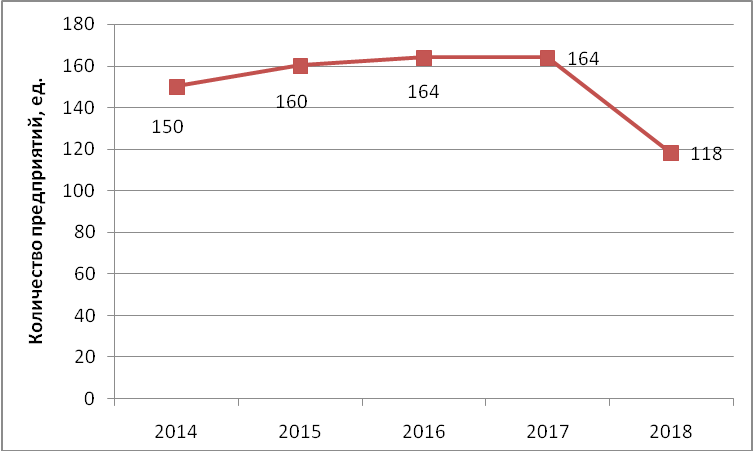
\includegraphics[width=1\textwidth]{authors/serebryakova-fig-1.png}
  \end{center}

  \caption{Количество действующих строительных организаций по Магаданской
области за 2014--2018~гг.[3]}
  \label{fig:serebryakova-fig-1}
\end{figure}


Из рисунка видно, что за последние годы снизилось количество строительных организаций на 46 ед. Объем строительных работ, выполненный строительными организациями, представлен на рис.~2.

\begin{figure}[H]

  \begin{center}
    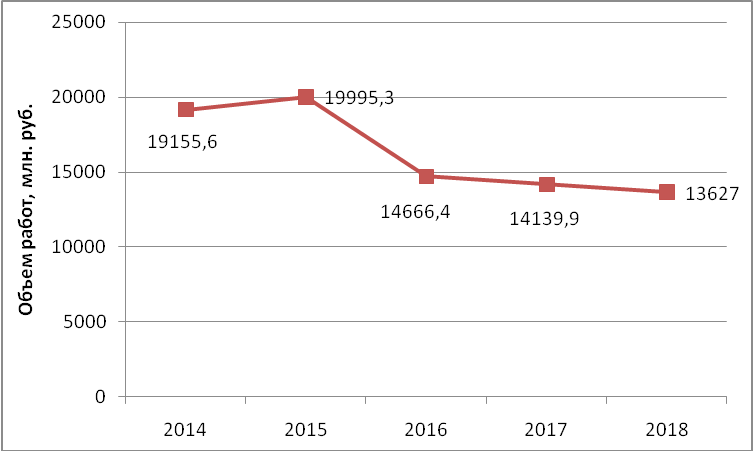
\includegraphics[width=0.8\textwidth]{authors/serebryakova-fig-2.png}
  \end{center}

  \caption{Объём строительных работ по Магаданской области
за 2014--2018~гг. [3]}
  \label{fig:serebryakova-fig-2}
\end{figure}


Рисунок свидетельствует также о снижении объёма строительных работ за последние годы на 513~млн~руб. Однако, темпы снижения строительных работ по сравнению с темпами снижения количества строительных организаций значительно ниже, из чего следует, что производительность труда в~строительных организациях остаётся на высоком уровне.

Объем строительных работ по Магаданской области за 2014--2018~гг., выполненных организациями различных форм собственности (млн~руб.) представлен в~таблице 1.

\begin{table}[h!]
\caption{Объем строительных работ по Магаданской области за 2014--2018~гг., выполненных организациями различных форм собственности (млн~руб.) [3]}
\label{tab:serebryakova-tab-1}
\begin{changemargin}{-2cm}{0cm}
\begin{tabular}{llllll}
\toprule
Форма 			собственности \newline строительной организации & 2014 			г. & 2015 			г. & 2016 			г. & 2017 			г. & 2018 			г. \\
\midrule
Государственная                                 & 114,1      & 32,0       & 82,1       & 1,5        & 0,3        \\
Муниципальная                                   & 321,9      & 170,4      & 125,8      & 183,5      & 150,9      \\
Частная                                         & 16114,7    & 18930,9    & 14454,8    & 13921,9    & 13213,3    \\
Смешанная 			российская                         & 141,5      & 75,6       & 3,8        & 33,0       & 0,2        \\
Совместная 			российская и иностранная          & 2463,4     & 786,4      & ---          & ---          & 262,3      \\
Итого                                           & 19155,6    & 19995,3    & 14666,4    & 14139,9    & 13627,0 \\
\bottomrule
\end{tabular}
\end{changemargin}
\end{table}


Таблица 1 свидетельствует, что доле частного бизнеса ежегодно принадлежит от~84 до 95\,\% всех выполненных строительных работ.

Основная цель региональных властей по удовлетворению потребности населения в~жилье~--- ввод в~действие жилых домов (рис.~3).

\begin{figure}[h!]

  \begin{center}
    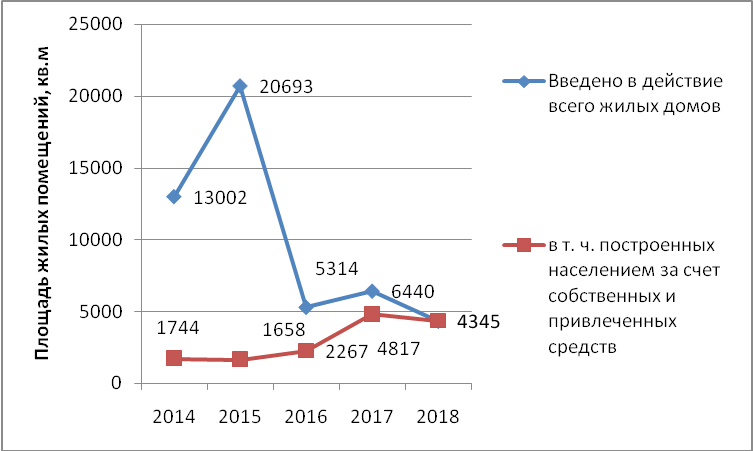
\includegraphics[width=1\textwidth]{authors/serebryakova-fig-3.png}
  \end{center}

  \caption{Ввод в действие жилых домов в Магаданской области
за 2014--2018~гг. [3]}
  \label{fig:serebryakova-fig-3}
\end{figure}

\vspace{-8pt}
Пик жилищного строительства в~2015~г. наблюдается ввиду того, что для возведения жилья были выделены средства из федерального и~регионального бюджета. Начиная с 2016~г. выделение средств из этих источников прекращено. Около 65 \,\%  площади жилых помещений возведено с привлечением частного капитала.

Наличие техники в~строительных организациях Магаданской области за 2014--2018~гг. представлено на рис.~4.

\begin{figure}[h!]

  \begin{center}
    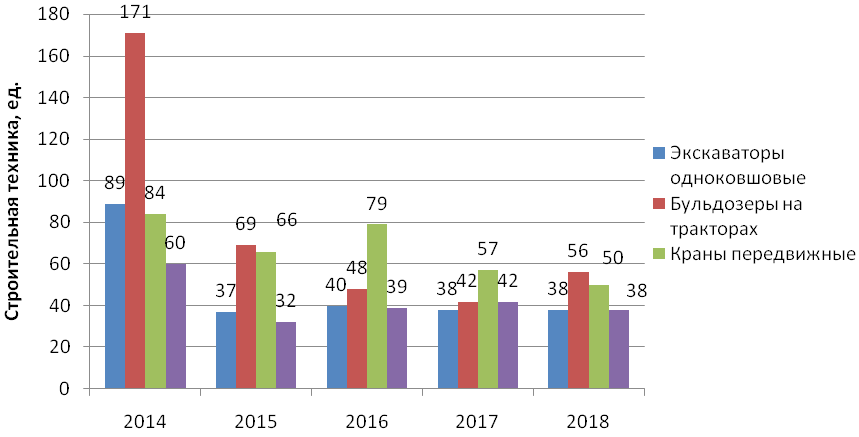
\includegraphics[width=1\textwidth]{authors/serebryakova-fig-4.png}
  \end{center}

  \caption{Наличие техники в строительных организациях Магаданской области
за~2014--2018~гг.}
  \label{fig:serebryakova-fig-4}
\end{figure}


Из рисунка видно, что за исследуемый период количество одноковшовых экскаваторов снизилось почти вдвое, бульдозеров~--- втрое. К тому же, одноковшовых экскаваторов с истекшим сроком службы до 40\,\%, кранов передвижных~--- 50\,\% и~выше [3].

Как видим, реализация стратегии массового жилищного строительства в~Магаданской области осуществляется в~сложных условиях, когда российская экономика переживает этап, на котором основные усилия государства направлены на модернизацию экономики, к тому же в~условиях слабой материально-технической базы.

Результаты выполнения плана жилищного строительства в~Магаданской области представлены в~таблице 2.

\begin{wraptable}{r}{7.0cm}

\caption{Результаты выполнения плана жилищного строительства в Магаданской области за 2014--2018~гг., м$^2$}
\label{tab:serebryakova-tab-2}
\begin{center}
\vspace{-8pt}

\begin{tabular}{cccc}
\toprule
Год  & План [2]  & Факт [3]  &  \parbox[c][][c]{0.1\textwidth}{ \centering \% вы\-пол\-не\-ния} \\
\midrule
2014 & 30000 & 13002 & 43            \\
2015 & 32000 & 20693 & 65            \\
2016 & 34000 & 5314  & 16            \\
2017 & 34000 & 6440  & 19            \\
2018 & 34000 & 4345  & 13\\
\bottomrule
\end{tabular}
\end{center}
\end{wraptable}


Данные таблицы свидетельствует о том, что идёт постепенное снижение жилищного строительства в~Магаданской области. Поэтому на региональном уровне требуется уделить внимание развитию инновационной инфраструктуры и~созданию эффективных институтов, способствующих коммерциализации научных идей и~разработок. Конечной целью внедрения инноваций на территории области является повышение эффективности деятельности существующих отраслей, а~также диверсификация экономики региона, снижение себестоимости и~расширение рынков сбыта производимой продукции.
\clearpage
Повышение конкурентоспособности экономики области во многом будет зависеть от~сроков и~эффективности найденного коммерческого применения инновационных разработок академической науки региона как имеющихся на сегодняшний день, так и~разработанных в~ближайшие годы.

Поиск возможностей коммерческого применения достижениям академической науки региона является первоочередной задачей на пути внедрения инноваций в~экономику. С целью решения этой задачи при научно-исследовательских институтах планируется создать ин\-но\-ва\-цион\-но-тех\-но\-ло\-ги\-чес\-кие отраслевые центры. В Северо-Восточном государственном университете для этой цели создана лаборатория стратегических и~инновационных исследований.

\begin{thebibliography}{99}
\bibitem{}Закон Магаданской области от 11 марта 2010 года №1241-ОЗ <<О стратегии социального и экономического развития Магаданской области на период до 2025 года>> (с изменениями на 18 марта 2019 года) // Docs.cntd.ru, все Кодексы РФ, СП, ГОСТ, Снип, Санпин, регламенты, указы, законы.~--- URL: http://docs.cntd.ru/document/895249692 (Дата обращения 10.03.2020).
\bibitem{}Постановление от 14 ноября 2013 г. № 1125-па <<Об утверждении государственной программы Магаданской области ,,Развитие предприятий промышленности строительных материалов, изделий и конструкций в Магаданской области‘‘ на 2014--2020 годы>> // Министерство строительства, жилищно-коммунального хозяйства и энергетики Магаданской области.~--- Системные требования: Adobe Acrobat Reader.~--- URL:
https://minstroy.49gov.ru/common/download.php?file=postanovlenie\_1125\_14.\\11.2013\_1.pdf\&obj=document (Дата обращения 10.03.2020).
\bibitem{}Статистический ежегодник. Магаданская область. 2014--2018. // Управление Федеральной службы государственной статистики по Хабаровскому краю, Магаданской области, Еврейской автономной области и Чукотскому автономному округу.~--- Системные требования: Архиватор Zip.~--- URL: http://habstat.gks.ru/folder/66943 (Дата обращения: 10.03.2020).

\end{thebibliography}
